\section{导论}

\subsection{The Three Elements of Computer Systems}
\begin{frame}
  \frametitle{\subsecname}
  \begin{columns}[c]
    \column{.5\textwidth}
    \begin{itemize}
      \item CPU 频率
        \begin{itemize}
          \item Multi-cores
          \item Multi-processers
          \item Multi-computers (Cluster)
        \end{itemize}
      \item Memory 大小
      \item IO
        \begin{itemize}
          \item Disk 容量,寻道传输比
          \item Network 带宽
        \end{itemize}
    \end{itemize}
    \column{.5\textwidth}
    \centering\framebox{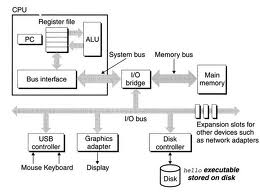
\includegraphics[scale=0.5]{images/three.jpeg}}
  \end{columns}
\end{frame}

\begin{frame}
  \frametitle{Process Model}
  \begin{columns}
    \column{.5\textwidth}
    \begin{itemize}
      \item Process
        \begin{itemize}
          \item Process
          \item Thread
        \end{itemize}
      \item \textcolor[rgb]{1.00,0.00,0.00}{IPC}
        \begin{itemize}
          \item Message Passing
          \item Shared Data
            \begin{itemize}
              \item Shared Memory
              \item Kernel Objects
              \item File
              \item Database
            \end{itemize}
        \end{itemize}
    \end{itemize}
    \column{.5\textwidth}
    \centering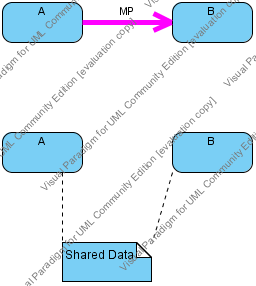
\includegraphics[scale=0.4]{images/ipc.png}\\
    \centering\textcolor[rgb]{0.00,0.00,1.00}{进程间通信机制}
  \end{columns}
\end{frame}

\begin{frame}
  \frametitle{Storage Hierarchy}
  \begin{itemize}
    \item \alert{Buffer}
    \item \alert{Cache}
  \end{itemize}

  \begin{figure}
    \centering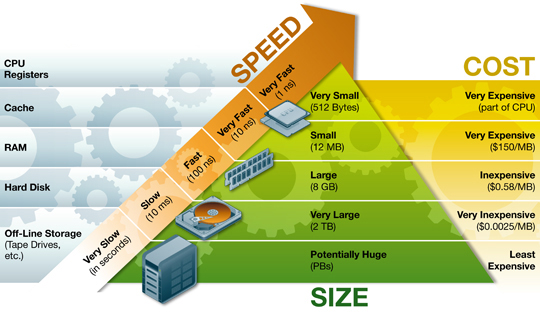
\includegraphics[scale=.5]{images/storage_hierarchy.jpg}
    \caption{Storage Hierarchy}
  \end{figure}
\end{frame}

\subsection{Distributed Systems}
\begin{frame}
  \frametitle{Distributed Systems}
  \fbox{\parbox{.9\textwidth}{Distributed system is an interconnected collection of autonomous computers, processes, or processors.}}
  \begin{columns}[t]
    \column{.5\textwidth}
    \begin{itemize}
      \item Information exchange
      \item Resource sharing
      \item Increased reliability through replication
      \item Increased performance through parallelization
      \item Simplification of design through specification
    \end{itemize}
    \column{.5\textwidth}
      \begin{enumerate}
        \item Process
        \item Communication
        \item Naming
        \item Sync
        \item Replication \& Cache
        \item Consistency
        \item Fault Tolerance
        \item Security
      \end{enumerate}
  \end{columns}
\end{frame}

\subsection{Parallel Computing}
\begin{frame}
  \frametitle{Parallel Computing}
  \begin{columns}
    \column{.5\textwidth}
    \begin{enumerate}
      \item Map
        \begin{itemize}
          \item 无法并行处理具有因果关系的任务
        \end{itemize}
      \item Reduce
    \end{enumerate}
    \column{.5\textwidth}
    \begin{figure}
      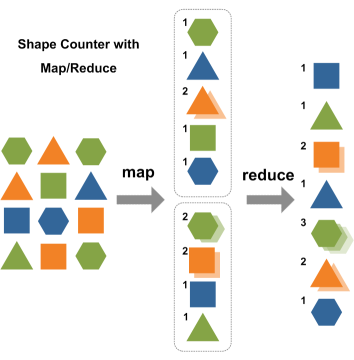
\includegraphics[scale=.4]{images/mapreduce_small.png}
      \caption{Map-Reduce}
      \label{mapreduce}
    \end{figure}
  \end{columns}
\end{frame}

\subsection{Virtualization}
\begin{frame}
  \frametitle{Virtualization}
  \begin{itemize}
    \item Server Virtualization
      \begin{itemize}
        \item 虚拟机作为一种隔离机制
        \item 虚拟机作为资源调度的单元
      \end{itemize}
    \item Storage Virtualization
      \begin{itemize}
        \item RAID
        \item NAS
        \item SAN
      \end{itemize}
    \item Network Virtualization
      \begin{itemize}
        \item VLAN
        \item VPN
      \end{itemize}
  \end{itemize}
\end{frame}

\subsection{Cloud Computing}
\begin{frame}
  \frametitle{\subsecname}
  \begin{itemize}
    \item Distributed Systems 
      \begin{itemize}
        \item Distributed File System
        \item Distributed Database (sql or nosql)
        \item Distributed Lock Server
      \end{itemize}
    \item Parallel Computing
      \begin{itemize}
        \item Map-Reduce Programming Model
      \end{itemize}
    \item Virtualization
    \item Cloud Management Platform
      \begin{itemize}
        \item Configuration \& Management \& Monitoring
        \item Load Balance
        \item Fault Tolerance
        \item Security
      \end{itemize}
  \end{itemize}
\end{frame}


\section{Software Engineering}
\subsection{Software Lifecycle Model}
\begin{frame}
  \frametitle{\subsecname}
  \begin{columns}[t]
    \column{.5\textwidth}
    \begin{figure}
      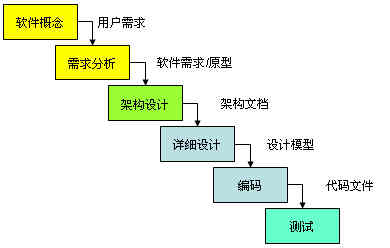
\includegraphics[scale=.3]{images/pubu.jpg}
      \caption{瀑布模型}
    \end{figure}
    \column{.5\textwidth}
    \begin{figure}
      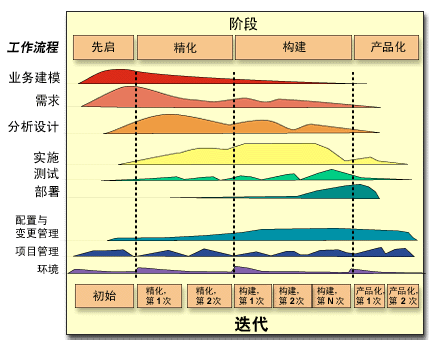
\includegraphics[scale=.2]{images/rup.png}
      \caption{Rational Unified Process}
    \end{figure}
    \begin{enumerate}
      \item 用例驱动
      \item 以基本架构为中心
      \item 迭代式和增量
    \end{enumerate}
  \end{columns}
\end{frame}

\subsection{Agile Programming}
\begin{frame}
  \frametitle{敏捷联盟12原则}
  \begin{enumerate}
    \item 尽早、持续交付有价值的中间软件使客户满意
    \item 即使到了开发后期,也欢迎需求变化,利用响应变化创造竞争优势
    \item 经常交付可工作的软件,间隔时间可以是几周到几个月,间隔越短越好
    \item 在开发全过程中业务人员和开发人员必须天天都在一起工作
    \item 为开发人员提供环境和支持,给予信任,以人为本地构建项目
    \item 团队内部最有效的沟通方式莫过于面对面的交谈
    \item 工作的软件是度量进度的最首要标准
    \item 提倡可持续的开发速度,责任人、开发者和用户应保持一个长期的、恒定的开发速度
    \item 不断关注好的技能和设计会增加敏捷能力
    \item 本质是简单--使未完成的工作最大化的艺术
    \item 自组织的团队才能做出最好的架构设计和需求分析
    \item 团队应定期在如何更有效工作方面进行反省,然后对自己的行为作出改进
  \end{enumerate}
\end{frame}

\begin{frame}
  \frametitle{主要的敏捷方法}
  \begin{itemize}
    \item<+-> 水晶方法 (Crystal)
    \item<+-> Dynamic System Development Method (DSDM)
    \item<+-> Feature-Driven Development (FDD)
    \item<+-> Adaptive Software Development (ASD)
    \item<+-> Scrum
    \item<+-> \alert{eXtreme Programming (XP)}
  \end{itemize}
\end{frame}

\begin{frame}
  \frametitle{XP的12条最佳实践}
  \begin{enumerate}
    \item 计划游戏
    \item \alert{小型发布}
    \item 隐喻
    \item 简单设计
    \item \alert{测试先行}
    \item \alert{重构}
    \item 结对编程
    \item 集体代码所有制
    \item \alert{持续集成}
    \item 每周工作40小时
    \item 现场客户
    \item 编码标准
  \end{enumerate}
\end{frame}

\subsection{Coding and Test}
\begin{frame}
  \frametitle{开发和测试的关系}
  \centering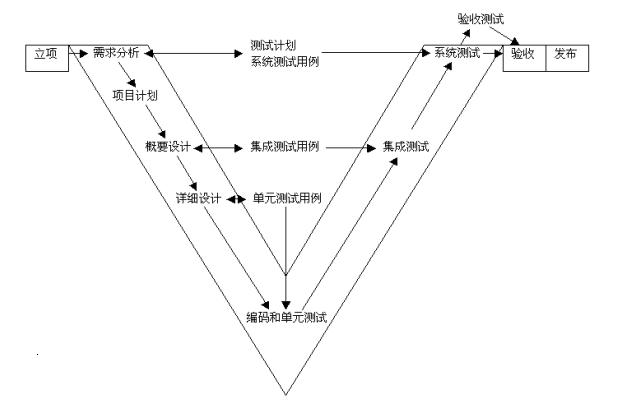
\includegraphics[scale=.4]{images/test.jpg}
  \begin{block}{Test-Driven Development}
    \small TDD是极限编程的重要特点,对接口设计,代码质量有促进作用。\\ 
    %\href{http://www.ibm.com/developerworks/cn/linux/l-tdd/}{\beamerbutton{tdd}}
    \url{http://www.ibm.com/developerworks/cn/linux/l-tdd/}
  \end{block}
\end{frame}

\subsection{Summary}
\begin{frame}
  \frametitle{Key Concepts}
  \begin{itemize}
    \item Use Case
    \item Architecture
  \end{itemize}
\end{frame}

\begin{frame}
  \frametitle{Architecture}
  \begin{itemize}
    \item 一个二重性的定义: 模块及模块之间的交互关系。
      \begin{itemize}
        \item 水平划分
        \item 垂直划分
      \end{itemize}
    \item 4+1视图
      \begin{enumerate}
        \item 物理视图
        \item 逻辑视图
        \item 开发视图
        \item 运行视图
        \item \alert{用例视图}
      \end{enumerate}
  \end{itemize}
  \begin{block}{讨论}
    \alert{正交性}
  \end{block}
\end{frame}


\section{Programming Languages}
\begin{frame}
\frametitle{The Evolution of Programming Languages}
\begin{itemize}
  \item 1GL 机器语言
  \item 2GL 汇编语言
  \item \alert{3GL}
    \begin{itemize}
      \item C/C++
      \item Java
      \item Python
      \item Elrang
    \end{itemize}
  \item 4GL+
\end{itemize}
\end{frame}

\begin{frame}
  \frametitle{二重性:数据+过程}
  \begin{columns}
    \column{.5\textwidth}
    \begin{itemize}
      \item 数据抽象
        \begin{itemize}
          \item 简单数据类型
          \item 复合数据类型
          \item Container
        \end{itemize}
      \item 过程抽象
        \begin{itemize}
          \item Function
        \end{itemize}
      \item 对象:统一数据和过程
        \begin{itemize}
          \item Object
          \item Message
        \end{itemize}
    \end{itemize}
    \column{.5\textwidth}
  \end{columns}
\end{frame}

\begin{frame}
  \frametitle{Language Paradigms}
  \begin{description}[面向对象语言]
    \item [命令式语言] 以Turing Machine为基础,计算被视为动作的序列,代表语言有C
    \item [函数式语言] 以$\lambda$-演算为基础,函数是一种对应规则,一定的输入参数产生唯一的输出,代表语言有Lisp, Haskell,Erlang
    \item [面向对象语言] 对象是要进行建模的任何事物,具有状态和操作,代表语言有C++,Java
    \item [逻辑式语言] 以形式逻辑为基础,代表语言有Prolog(Programming in Logic)
  \end{description}
\end{frame}

\subsection{Imperative Programming}
\begin{frame}
  \frametitle{Imperative Programming}
  statements1;\\
  statements2;\\
  \dots
\end{frame}

\subsection{Functional Programming}
\begin{frame}[t]
  \frametitle{Functional Programming}
  \begin{definition}
    $function_n(\cdots function_2(function_1(data))\cdots)$
  \end{definition}

  引起副作用的操作:
  \begin{itemize}
    \item 全局状态
    \item IO
    \item Network Communication 
  \end{itemize}
\end{frame}

\begin{frame}
  \frametitle{Concurrency-Oriented Programming}
  \begin{itemize}
    \item 轻量级进程
    \item 进程间通过消息进行通信
  \end{itemize}
\end{frame}

\begin{frame}[containsverbatim]
  \frametitle{Case Study: Erlang}
  \begin{block}{Erlang Features}
    \begin{itemize}
      \item Functional Programming
      \item Concurrent Programming
      \item Distributed Systems
      \item Fault tolerance
    \end{itemize}
  \end{block}

  \begin{verbatim}
  -module(fib).
  -export([fib/1]).

  fib(0) -> 0;
  fib(1) -> 1;
  fib(N) when N > 1 ->
      fib(N-1)+fib(N-2).
  \end{verbatim}
\end{frame}

\subsection{Object-Oriented Programming}
\begin{frame}
  \frametitle{Object-Oriented Programming}
  \begin{itemize}
    \item 封装: 统一状态和操作,面向接口
    \item 继承: 重用已有类,扩展,重定义\\
      {\centering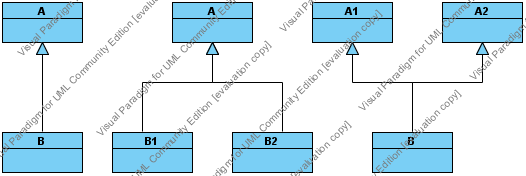
\includegraphics[scale=0.4]{images/class.png}}
    \item 多态: 一样的接口,不一样的行为
  \end{itemize}
  \begin{block}{面向接口编程}
    设计一致的接口,保持接口的相对稳定性,对代码质量的提升有巨大的价值。
  \end{block}
\end{frame}

\begin{frame}[containsverbatim]
  \frametitle{Case Study}
  \begin{columns}[t]
    \column{.5\textwidth}
    \begin{alltt}
    class A \{
    public:
      \alert{A();}\footnote{Object Lifecycle}
      \alert{virtual ~A();}
      \alert{virtual print() const;}\footnote{虚函数}
      int get_a() const;
      void set_a(int a);
    private:
      int ma;
    \};
    \end{alltt}
    \column{.5\textwidth}
    \begin{alltt}
    class B : \alert{public A} \{
    public:
      \alert{B();}
      \alert{virtual ~B();}
      \alert{virtual print() const;}
    private:
      int mb;
    \};
    \end{alltt}
  \end{columns}
\end{frame}

\begin{frame}
  \frametitle{How to implement OO using C?}
  \begin{figure}
    \centering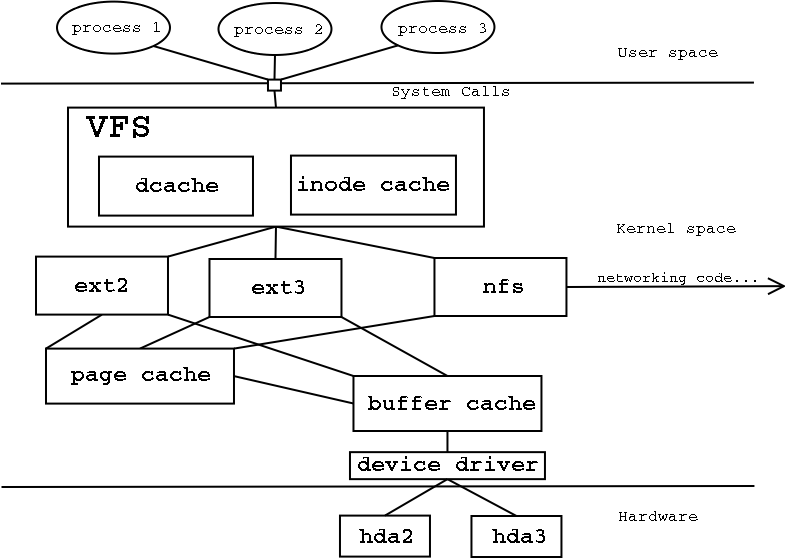
\includegraphics[scale=.3]{images/vfs_relations_static.png}
    \caption{vfs relations}
  \end{figure}
\end{frame}

%\subsection{Logic Programming}
%\begin{frame}
%  \frametitle{Prolog}
%  enabling condition1 $\rightarrow$ action1\\
%  enabling condition2 $\rightarrow$ action2\\
%  \dots
%\end{frame}

%%%%%%%%%%%%%%%%%%%%%%%%%%%%%%%%%%%%%%%%%%%%%%%%%%%%%%%%%%%%%%%%%%%%%%%%
\section{The Pragmatic Programmer}
\subsection{Mastering 1+ Programming Languages}
\begin{frame}
  \frametitle{\subsecname}
  \begin{columns}[t]
    \column{.5\textwidth}
    Programming Languages:
    \begin{itemize}
      \item<+-> \alert{C}/C++/Java
      \item<+-> \alert{Python}/Perl/PHP/Ruby
      \item<+-> \alert{Erlang}/Scala
      \item<+-> Shell
    \end{itemize}
    \column{.5\textwidth}
    Tools (IDE):
    \begin{itemize}
      \item Editor
      \item Compiler
      \item Build System
      \item Version Control System
      \item Debugger
      \item Profiler
    \end{itemize}
  \end{columns}
\end{frame}

\begin{frame}
  \frametitle{Clean Code}
  \begin{block}{Ron Jeffris}
    近年来,我开始研究Beck的简单代码规则,差不多也都琢磨透了。简单代码,依其重要顺序:
    \begin{itemize}
      \item 能通过所有测试
      \item 没有重复代码
      \item 体现系统中的全部设计理念
      \item 包括尽可能少的实体,比如类、方法、函数等
    \end{itemize}
  \end{block}
\end{frame}

\begin{frame}
  \frametitle{系统结构设计原则}
  \begin{description}[自顶向下,逐步求精]
    \item [自顶向下,逐步求精] 抓住系统总的功能目的,然后逐层分解
    \item [高内聚、低耦合] 模块内部组合要尽可能紧凑,模块之间的耦合要尽可能小
    \item [信息隐藏] 只暴露必要的接口,隐藏具体实现细节
    \item [单一职责原则]
    \item [依赖倒置原则]
    \item [开放封闭原则]
  \end{description}
\end{frame}

\begin{frame}
  \frametitle{Function Design Principles}
  \begin{itemize}
    \item 函数的第一规则是要短小,第二条规则是还要更短小
    \item 函数应该做一件事,做好这件事,只做这一件事
    \item 最理想的参数数量是零个,其次是一,其次是二,应尽量避免三个及以上
    \item 无副作用
  \end{itemize}
\end{frame}

\begin{frame}
  \frametitle{Class Design Principles}
  每个达到一定规模的系统都会包含大量逻辑和复杂性。管理这种复杂性的首要目标就是\textcolor{red}{加以组织},
  以便开发者知道到哪儿能找到东西,并且在某个特定时间只需要理解直接有关的复杂性。 
  反之,拥有巨大、多目的类的系统,总是让我们在目前并不需要了解的一大堆东西中艰难跋涉。
\end{frame}

\subsection{Reading the Fucking Source Code}
\begin{frame}
  \frametitle{\subsecname}
\end{frame}

\subsection{Understanding Patterns}
\begin{frame}
  \frametitle{\subsecname}
  \begin{itemize}
    \item Data Structures and Algorithms
    \item Design Patterns
    \item Architecture Patterns
  \end{itemize}
\end{frame}

\subsection{Understanding Requirements}
\begin{frame}
  \frametitle{\subsecname}
\end{frame}

%%%%%%%%%%%%%%%%%%%%%%%%%%%%%%%%%%%%%%%%%%%%%%%%%%%%%%%%%%%%%%%%%%%%%%%%
\section{The Duality of World}
\begin{frame}
  \frametitle{一些矛盾}
  \begin{tabular}{c|c}
    +           & - \\ 
    \hline
    \hline
    虚          & 实 \\
    合          & 分 \\
    动          & 静 \\
    Software    & Hardware \\
    \hline
    简单        & 复杂 \\
    个人        & 团队 \\
    自由        & 纪律 \\
    Development & Test \\
    \hline
    Language    & Machine \\
    Data        & Function \\
    Local       & Global \\
    Pure        & Dirty \\
    \hline
    实践        & 理论
  \end{tabular}
  \begin{block}{讨论}
    \alert{分界线在哪儿?}
  \end{block}
\end{frame}

\begin{frame}
  \frametitle{研究二元关系的哲学}
  \begin{description}[辩证发展观]
    \item [辩证发展观] 迭代式、螺旋上升
    \item [易之三义] 变易、不易、简易
  \end{description}
  \hrule
  \begin{columns}[b]
    \column{.5\textwidth}
    \begin{figure}
      \centering
\includegraphics[scale=.35]{images/taiji.jpg}
      \caption{太极图}
      \label{taiji}
    \end{figure}
    \column{.5\textwidth}
    \begin{figure}
      \centering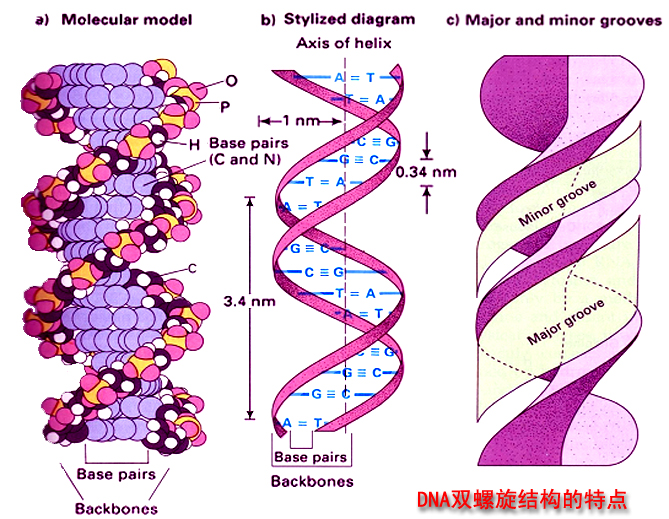
\includegraphics[scale=.25]{images/dna.jpg}
      \caption{双螺旋结构}
      \label{dna}
    \end{figure}
  \end{columns}
\end{frame}

\begin{frame}
  \frametitle{研究二元关系的数学工具}
  \begin{columns}
    \column{.5\textwidth}
    \begin{itemize}
      \item Bool Algebra
      \item Graph Theory
      \item Petri Net
      \item Finite State Machine
    \end{itemize}
    \column{.5\textwidth}
    \begin{figure}
      \centering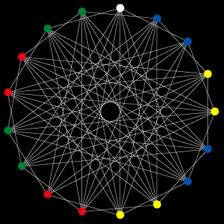
\includegraphics[scale=.5]{images/graph.jpeg}
      \caption{A Graph}
    \end{figure}
  \end{columns}
\end{frame}

\begin{frame}
  \frametitle{The End}
  \begin{center}
    {\Huge 谢谢大家!}
  \end{center}
\end{frame}
